% A字 例3：梯形 AD∥BC, 延长 BA,CD 交于 P, AD=4, BC=8, PA=5 求 AB=5
\documentclass[tikz,border=4pt]{standalone}
\usepackage{ctex}
\usepackage{amsmath}
\usetikzlibrary{calc}
\begin{document}
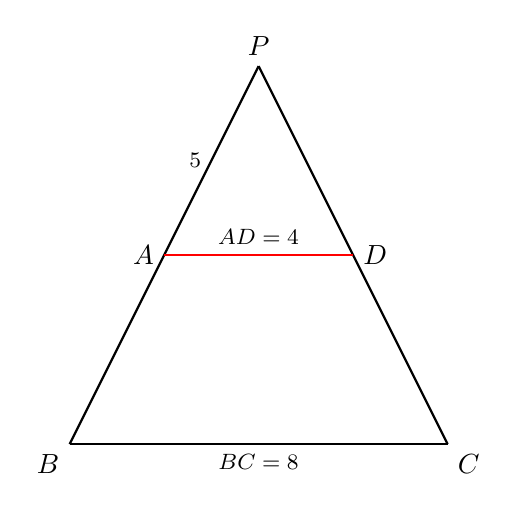
\begin{tikzpicture}[scale=0.6, thick]
  % 顶点 P 上方. PB=10, PC=10 (对称). 上底 AD=4 中点正下方 P
  \coordinate (P) at (0,8);
  \coordinate (B) at (-4,0);
  \coordinate (C) at (4,0);
  % A 在 PB 上, PA=5, PB=10 -> A=P + 0.5*(B-P) = (-2,4)
  \coordinate (A) at ($(P)!0.5!(B)$);
  \coordinate (D) at ($(P)!0.5!(C)$);
  \draw (P)--(B);
  \draw (P)--(C);
  \draw (B)--(C);
  \draw[red] (A)--(D);
  \node[above] at (P) {$P$};
  \node[left] at (A) {$A$};
  \node[right] at (D) {$D$};
  \node[below left] at (B) {$B$};
  \node[below right] at (C) {$C$};
  \node[above] at ($(A)!0.5!(D)$) {\footnotesize $AD=4$};
  \node[below] at ($(B)!0.5!(C)$) {\footnotesize $BC=8$};
  \node[left] at ($(P)!0.25!(B)$) {\footnotesize $5$};
\end{tikzpicture}
\end{document}
